\chapter{SCR Models for Open Populations}
\markboth{Open Populations}{}
\label{chapt.open}


\vspace{0.3cm}


\section{Introduction}

All of the previous chapters focused on closed population models
for estimating density and for inference about spatial variation in density. 
However, a thorough
understanding of population dynamics also requires information about both
spatial and temporal variation in population density and demographic parameters. 
In this chapter,
we develop a framework for
inference about the processes governing spatial and temporal dynamics,
namely survival, recruitment, and movement (migration, dispersal, etc...).
The ability to estimate these parameters is critical to both basic and
applied ecological research. For example, testing hypotheses about
life history trade-offs requires accurate estimates of both survival
and fecundity (citations). Inference about density-dependent population
regulation, which has fascinated theoretical ecologists for well over
a century, is likewise best accomplished by studying
the factors affecting survival and fecundity, rather than the more common approach of
modeling time series data \citep{nichols_etal:2000}.  Modeling vital
rates is just as important for applied ecologists and conservation
biologists, because a mechanistic understanding of population decline
and requires it. Furthermore, if we know how environmental
variables affect demographic parameters, we can make predictions about
population changes under different future scenarios. We can also assess
the sensitivity of parameters such as population growth rate to
variation in survival or fecundity. Although matrix
population models are often used for these purposes \citep{caswell:1989,saether_bakke:2000}, the same
objectives can be accomplished by computing posterior predictive
distributions as part of the MCMC algorithm.

For the first time, we can fully
integrate the movement of individuals onto and off of the trap array
with their encounter histories to simultaneously estimate density,
survival, and recruitment in a spatial model.  For many species, such
as those that are rare or not often observed by researchers, this allows us
to make inference about survival and recruitment without having
to physically capture individuals.  Additionally, another reason
extending our SCR models to open populations arises purely from a
sampling perspective.  We often need longer time periods to sample
rare or elusive species to ensure that enough captures and recaptures
are produced.  This extended time frame can quickly lead to violations
in the assumption of population closure.  For example, the European
wildcat study that was presented in chapter XXX insert ref XXX was
conducted over a year long period.  While the researchers in that
study used a closed population, they did model variation in detection
as a function of time.  Another approach would have been to use an
open population model (the spatial capture recapture open models had
not been developed at the time of the wildcat study, so we'll forgive
the authors for not having used this more appropriate model).

The modeling framework we will develop in this chapter is based on a
formulation of Cormack-Jolly-Seber (CJS) and Jolly-Seber (JS) type
models \citep{cormack:1964, jolly:1965, seber:1965} that are amenable
to modeling individual effects, including individual covariates.
There is a long history of use of these models in fisheries, wildlife,
and ecology studies \citep{pollock_etal:1990, lebreton_etal:1992,
  pradel:1996, williams_etal:2002, schwarz_arnason:2005,gimenez:2007}.
Additionally, there have been many modifications and developments of
the CJS and JS models including dealing with transients, multi-state,
and spatially implicit models.

\subsection{Overview of Population Dynamics}

The most basic formulation of models for population growth stem from an idea originally used
in accounting, the balance sheet.  In this case, we can think of the population as a function
of credits (i.e., births and immigrants) and debits (i.e., deaths and emigrants).  We can then
set up the population at time $t+1$ as a function of these four components:
\[
N(t+1) = N(t) + B(t) + I(t) - D(t) - E(t)
\]
where $N(t)$ is the population size at time $t$, $B(t)$ and $I(t)$ are the credits (additions) from births and
immigrants at time $t$, and $D(t)$ and $E(t)$ are the debits (losses) due to deaths and emigration.   This balance
equation model is then termed the "BIDE model".  We can easily derive
a simple population growth model under density independence, by assuming no immigration or emigration.
\[
N(t+1) = N(t) + N(t)r(t)
\]
where $r(t) = b(t) - d(t)$.  Here, $b(t)$ and $d(t)$ are the per-capita birth and death rates and thus $r(t)$ is the per-capita
growth rate.  Density-dependent, age structured, stochastic effects on growth, spatially structured, and competition models (e.g.,Lotka-Volterra)
all are basic derivations of the BIDE model.

In closed population models, we focus on estimating $N(t)$, but in open population models
we are interested in the dynamics that arise between years or seasons and thus we focus not only on $N(t)$ but on these so-called ``credits'' and 
``debits" that drive the population changes. If we take the basic parameters in the BIDE model and reconceptualize them,
we can relate these to the commonly used parameters in JS and CJS models, described in more detail below.
For example, survival ($\phi(t)$) is defined as the probability of an individual surviving from time $t$ to $t+1$, and often we call this '$apparent$ survival' because deaths and emigration cannot be separated. Mortality, the probability of dying from time $t$ to $t+1$, is $1-\phi(t)$.
Recruitment ($\gamma$) is the probability of a new individual entering the population between $t$ to $t+1$, which includes those both those
born into the population and immigrants.


\subsection{Animal movement related to population demography}

We commonly consider that density may influence demographic parameters such as
survival rates, population growth, etc., it is also likely that movement of individuals
can influence these parameters.  For example, we know that movement of transients will affect
our estimates of survival, causing us to typically refer to estimates as ``apparent survival".
This is because an animal that appears in the population for a short period of time and then leaves
is going to appear as though it has died.  Due to this problem, there has been a significant amount
of work developing models to deal with transients in both closed and open capture-recapture models
\citep{kendalletal:1997, pradeletal:1997, hinesetal:2003, claveletal:2008}.  Because we estimate movement
within the SCR framework, we can better understand the impact of animals moving onto and off of the trap
array and hence we can improve our estimates of survival by combining the traditional CJS and JS models with
the SCR model.

But
what if movement and space usage of individuals directly influences the survival rates or recruitment?
It is generally accepted that population structure (i.e., age, stage, or size distribution) can affect
 both population size and growth over time.  We also know that how animals associate themselves in space
can directly influence the age or stage structure of a population -- this can be behavioral, habitat
related, or some combination of factors.  For example, if habitat is limited and we have a territorial
 species, then we might expect that some younger members of the population might have trouble finding
and/or defending a territory.  Ultimately, this may lower survival for a certain age class in the population directly
impacting the population structure.  We also understand that there are impacts on the population structure from animals
dispersing.  In many
animal populations, dispersal is linked with reproduction and population regulation.  Thus, movement including spatial
arrangement of activity centers and dispersal are key components to population dynamics. We start here by showing
how to extend the SCR models to open populations, but this chapter opens the door for how we would go about
incorporating space usage into models of demographic dynamics.  For example, we could incorporate space and movement
into age-dependent multistate capture-recapture models to address
the impact of dispersal on recruitment or survival.



\subsection{Basic assumptions of JS and CJS models}

Before extending the classic open models to our SCR framework, let's first look
at the basic assumptions of both models.  No tag (or mark) loss is
assumed in both models.  If a marked animal losses it's tag or
mark, then that animal cannot be recaptured and this could appear as
though the animal has died.  Hence, to maintain unbiased estimates of
survival, no tag or mark loss is important.  Additionally, capture and
release should be instantaneous (or as close as possible), otherwise
the time interval between capture occasions could differ for
individuals and that would result in individual heterogeneity of
survival.  Individuals must also be recorded accurately.

In the standard CJS models, it is also assumed that all emigration
from the study area is permanent and that capture and survival
probabilities are constant within each sample occasion and group.  A
group can be created based on sex, age, area, etc.  In the CJS
formulation of the model, we condition on the captured individuals,
and therefore we estimate only the probability of recapture and the survival
rates.  Here, survival is considered the ``apparent'' survival because
emigration and mortality are confounded within the model, thus
apparent survival is always estimated lower than true survival when
emigration is not zero.  In the JS version of the model, we do not
condition on marked individuals.  Thus we can estimate survival like
we do in the CJS, but now we can also model recruitment (new
individuals coming into the population) and the total
abundance/density of the population.  Estimating more parameters does
require a few more assumptions including that all individuals in the
population have the same probability of capture.  Under a ``robust
design'' (\citep{pollock:1982}, which we will demonstrate in this
chapter, we can estimate heterogeneity in capture probabilities.



\section{Traditional Jolly-Seber Models}

There are a number of ways that researchers have used to formulate the JS model and while
all of these models are slightly different parameterizations of the underlying population processes,
they are all essentially equivalent.  The resulting estimates of abundance and the driving parameters such
as survival and some form of recruitment should be the same.  The most commonly used formulations are the
Link-Barker, Pradel-recruitment, Burham JS, and the Pradel-l models. In all of these models, we are interested
in recruitment, or how new individuals arrive into the population.  Therefore one the main differences between
the various models is how new entrants into the population are parameterized.

Pollock (1982) created the robust design in order to allow for heterogeneity in capture probability
under the JS model.  The basic idea is that there are primary occasions (e.g., years, seasons) and we
allow the population to be "open" between the primary occasions.  This means that individuals can enter
and leave the population (i.e., births, deaths, immigration, emigration) between the primary occasions.
However, within a primary occasion, the population is assumed to be closed to these processes.  Typically,
the JS sampling framework would not allow for variation in detection probability between individuals or within
a primary occasion because only one sample was taken. However, when multiple samples are taken within a primary
occasion (we call these ``secondary occasions"), then variation in detection probability can be modeled and thus
our estimates of $N$ can be improved.  To
that extent, we can envision the data as arising from repeated
sampling over seasons or years (or {\it primary} periods) within which
one or more samples (e.g., nights) might be taken ({\it secondary}
periods). Fig. \ref{open.figs.robustdesign} demonstrates the sampling process graphically. Comparing this with all of our previous work, the sample
intervals (e.g., trap nights, weeks, etc. ) described in the closed
population chapters are equivalent to {\it secondary} periods).

\begin{figure}
\centering
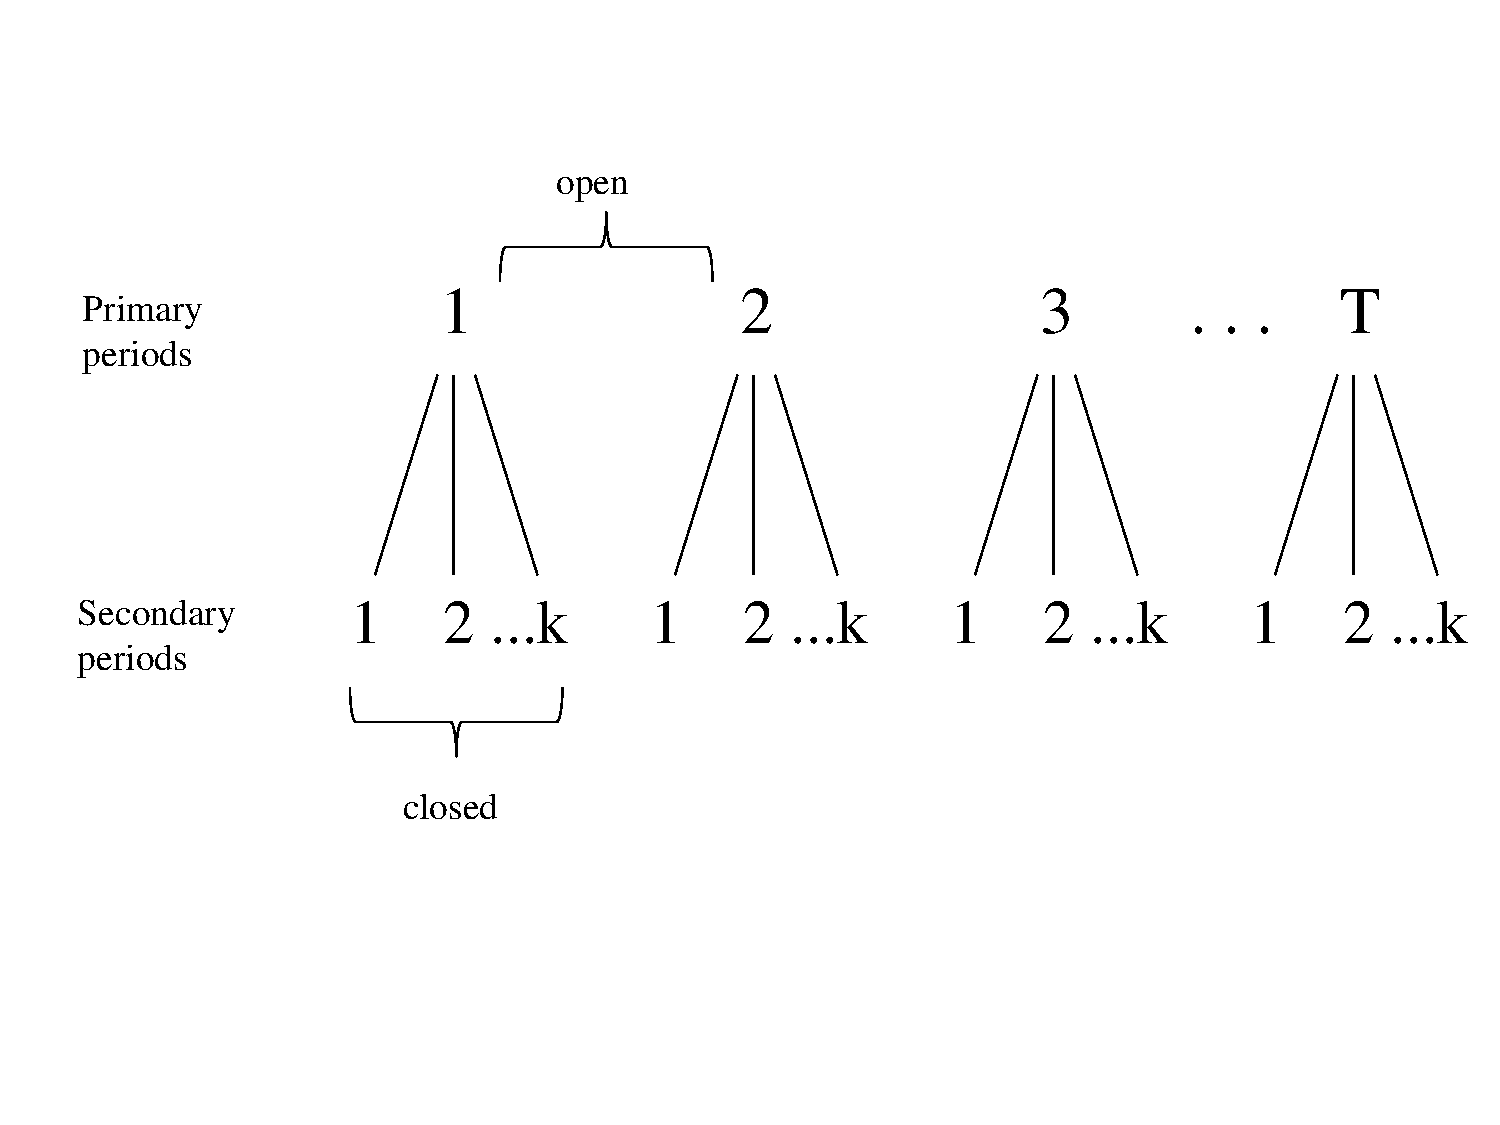
\includegraphics[height=2in,width=2.5in]{Ch12/figs/RobustDesign.pdf}
\caption{Schematic of the robust design with T primary sampling periods and K secondary periods. The populations
are considered open between primary periods and closed within the secondary}
\label{open.figs.robustdesign}
\end{figure}

Based on the robust design, we can easily create a non-spatial JS model.  We define $y_{ikt}$ as the encounter
history for individual $i$ at secondary occasion $k$ during primary occasion $t$.  If we have a Bernoulli encounter
process then we can describe the observation model, specified conditional on $z(i,t)$, as:
 \[
  y_{ikt}|z(i,t) \sim
\mbox{Bernoulli}(p z(i,t)).
\]
Thus, if individual $i$ is alive at time $t$ ($z(i,t)=1$), then the
observations are Bernoulli with detection probability $p$ as before.  Conversely, if the individual is
not alive ($z(i,t)=0$), then the observations must be fixed zeros with
probability 1.

Survival and recruitment in the open population are manifest in a
model for the latent state variables $z(i,t)$ describing individual
mortality and recruitment events.  An important aspect of the
hierarchical formulation of the model that we adopt here is that the
model for the state variables is described conditional on the total
number of individuals ever alive during the study (a parameter which
we label $N$) based on $T$ periods, as in \cite{schwarz1996gma}.  Data
augmentation induces a special interpretation on the latent state
variables $z(i,t)$.  In particular, ``not alive'' includes individuals
that have died, or individuals that have not yet been recruited.
Using this formulation simplifies the state model and also allows it
to be implemented directly in the JAGS software \cite {royle:book}.
For example, considering the case $T=2$, the state model is composed
of the following two components: First the initial state is described
by:
\[
 z(i,1) \sim \mbox{Bern}(\psi)
\]
and then a model describing the transition of individual states from
$t=1$ to $t=2$:
\[
 z(i,2) \sim \mbox{Bern}( \phi z(i,1)  + \gamma (1-z(i,1)) ).
\]
If $z(i,1)=1$, then the individual may survive to time $t=2$ with
probability $\phi$ whereas, if $z(i,1)=0$, then the
``pseudo-individual'' may be recruited with probability $\gamma$.

We can then generalize this model for $T>2$ time periods and allow survival and
recruitment to be time dependent.  Initialize the
model for time $T=1$ as we have done above
and then the model describing the transition of individual states from
$t$ to $t+1$ is:
\[
 z(i,t+1) \sim \mbox{Bern}( \phi_t z(i,t)  + \gamma_t (1-z(i,t)) ).
\]

This parameterization then results in $T-1$ survival and recruitment
parameters.  The main difference here from the CJS model, described below,
 is that we include recruitment and are interested in estimating $N$ for each $t$.
Since this state model described above is conditional-on-N, we must
deal with the fact that N is unknown, which is done through data
augmentation similar to how we used it in the closed population models.


\subsection{Data Augmentation for the Jolly-Seber Model}

The fundamental challenge in carrying out inference under this model
is that the parameter $N$ (the total number of individuals alive
during at least 1 time period) is not known.  We have discussed and
demonstrated data augmentation in many previous chapters; however,
with the open population model, we have to take care that two issues
are addressed: 1. the data augmentation is large enough to accommodate
all potential individuals alive in the population during the entire
study and 2. that individuals cannot die and then re-enter the
population.  To begin, let's consider the role of $\gamma$ in the
model.

Data augmentation formally reparameterizes the model, replacing $N$,
the number of individuals ever alive with the parameter $\psi$ which
is interpretable as the population size expressed as a fraction of
$M$.  That is, the expected value of $N$ under the model is equal to
$\psi M$.  As a result of this repararameterization, the recruitment
parameters $\gamma_{t}$ are also relative to the number of ``available
recruits'' on the data augmented list of size $M$, and not directly
related to the population size.  This is easily resolved by deriving
$N_t$, and $R_{t}$, the population size and number of recruits in year
$t$, as a function of the latent state variables $z(i,t)$.  In
particular, the total number of individuals alive at time $t$ is
\[
N_{t} = \sum_{i=1}^{M} z(i,t)
\]
and the number of recruits is
\[
R_{t} = \sum_{i=1}^{M} (1-z(i,t-1))z(i,t)
\]
which is the number of individuals {\it not} alive at time $t-1$ but
alive at time $t$.

In the case of just two primary periods, this process is
straightforward.  When the number of primary sample occasions is
greater than 2, we must formulate the model for recruitment by
introducing another latent variable.  We do this in order to ensure
that an individual can only be recruited once into the population.
Here, this formulation of the model uses a set of latent indicator
variables $r(i,t)$ which describe the time interval $(t-1, t)$ at
which individual is recruited into the population.  Let $r(i,t) = 1$
if individual $i$ is recruited in time interval $(t-1, t)$ otherwise
$r(i,t)=0$.  To construct the recruitment process we make use of the
standard conditional binomial construction of a removal process
(\citealt{royle:book}).  The initial state is given by:
\[
   r(i,1) \sim \mbox{Bin}(1, \gamma_{1})
\]
for $i=1,2,\ldots,N$. Then, for $t>1$
\[
 r(i,t)|r(i, t-1) \dots r(i, 1) \sim \mbox{Bin}((1 - \sum_{\tau=1}^{t-1} r(i, \tau) ) \times \gamma_{t}, 1)
\]
Each recruitment variable is conditional on whether the individual was ever
previously recruited and this construction forces the recruitment
variable after initial recruitment to be degenerate (have a sample
size of 0).  Then, we can describe the state variables $z(i,t)$ by a
1st order Markov process.  For $t=1$, the initial states are fixed:
\[
z(i,1) \equiv r(i,1)
\]
and,
 for subsequent states, we have
\[
z(i,t)|z(i,t\,-\,1),r(i,t)
 \sim \mbox{Bern} (\phi_{t} z(i,t\,-\,1)) \,+ \,  r(i,t).
\]
Thus, if an individual is in the population at time $t$ (i.e., $z(i,t)
= 1$), then that individual's status at time $t+1$ is the outcome of a
Bernoulli random variable with parameter (survival probability)
$\phi_{t}$.  If the individual, however, is not in the population at
time $t$ (i.e., $z(i,t) = 0$), then the outcome is a Bernoulli random
variable with probability $\gamma_{t}$, a parameter that is related to
{\it per capita} recruitment.  We carry out this process in \jags~ by
using the \mbox{\tt sum}() and \mbox{\tt step}() functions together to
ascertain if a particular individual $i$ was ever previously alive.
Individuals that were ever previously alive are no longer eligible to
be ``recruited" into the population.  The implementation of this model
in \jags~ is shown in panel \ref{open.panel.nsJS}.


\begin{panel}[htp]
\centering
\rule[0.1in]{\textwidth}{.03in}
{\small
\begin{Verbatim}[commandchars=\\\{\}]
model\{

psi \mytilde dunif(0,1)
phi \mytilde dunif(0,1)
p.mean \mytilde dunif(0,1)

for(t in 1:5)\{
N[t] <- sum(z[1:M,t])
gamma[t] \mytilde dunif(0,1)
\}

for(i in 1:M)\{
  z[i,1] \mytilde  dbern(psi)
 cp[i,1] <- z[i,1]*p.mean
  Y[i,1] \mytilde  dbinom(cp[i,1], K)
  a[i,1] <- (1-z[i,1])

for(t in 2:5)\{
      a1[i,t] <- sum(z[i, 1:t])          
       a[i,t] <- 1-step(a1[i,t] - 1)     

       mu[i,t]<- (phi*z[i,t-1]) + (gamma[t]*a[i,t-1])
        z[i,t] \mytilde dbern(mu[i,t])
       cp[i,t] <- z[i,t]*p.mean
        Y[i,t] \mytilde dbinom(cp[i,t], K)
         \}
        \}
\}
\end{Verbatim}
}

\rule[-0.1in]{\textwidth}{.03in}
\caption{
\jags~ model specification for the non-spatial JS model.}
\label{open.panel.nsJS}
\end{panel}



\subsection{Mist netting example}

We now return to the ovenbird data collected during a mist-netting
study, and initially presented in Chapt. \ref{chapt.poisson-mn}.  These data are available
in the \secr~ package (see, \citet{efford_etal:2004,
  borchers_efford:2008}). To refresh your memory: 44 mist nets spaced
30 m apart on the perimeter of a 600-m x 100-m rectangle (see
Fig. XXXX) were operated on 9 or 10 non-consecutive days in late May
and June for 5 years from 2005-2009.

In Chapt. \ref{chapt.poisson-mn}, we dealt with this dataset as a type of ``multi-season"
model where abundance in each year, $N_{t}$, was estimated
separately. This of course is a first step in thinking about data
collected over multiple years, but now, we can use the JS model to
estimate the demographic processes (survival and recruitment) between
years.

The first issue at hand is that each line in our 3-D encounter history
array of
data must correspond to a single individual.  Previously, we were not
interested in individual identity across years so this was not of
concern; however, we need to maintain the order of individuals across years
in order to estimate the survival and recruitment of the individual into the population.
We organize the data set so that each row in our
array represents just one individual across all primary periods.
For the ovenbird dataset, we
can organize the data by creating a master list of all individuals
captured during the entire study.  From this list, we can assign each
individual a unique row in our dataset (in the following R commands,
we do this by using the \mbox{\tt unique}() command on the row names
for each year of our 3-D array and use the command \mbox{\tt pmatch}()
to associate the data to the correct column).  Additionally, in
Chapt. \ref{chapt.poisson-mn} we carried out data augmentation for each year separately;
however, we must consider for example that individuals captured in
year $t$ could have been alive in year $t-1$.  Our data
augmentation must be large enough to include individuals alive during
any of the time periods and to account for that, we set M=200.  For this example,
we hold survival constant but allow recruitment to be time dependent
(since $\gamma$ is essentially a function of the data augmentation
process as described above, it does not make sense to hold recruitment constant and we 
therefore make it time specific).

{\small
\begin{verbatim}
library("secr")
library(scrbook)
data(ovenbird)

X<-traps<-traps(ovenCH)
xlim<-c(min(X[[1]][,1])-150,max(X[[1]][,1])+150)
ylim<-c(min(X[[1]][,2])-150,max(X[[1]][,2])+150)
ntraps<- nrow(traps[[1]])
Y<-ovenCH
K<-10
M<-200 # do constant data augmentation to all years
Sst<-cbind(runif(M,xlim[1],xlim[2]),runif(M,ylim[1],ylim[2]))
Sst<-array(Sst,dim=c(M,2,5))


hold<- unique(c(unlist(dimnames(Y[[1]])[1]), unlist(dimnames(Y[[2]])[1]),
       unlist(dimnames(Y[[3]])[1]), unlist(dimnames(Y[[4]])[1]),
       unlist(dimnames(Y[[5]])[1])))

Yarr<-array(ntraps+1,dim=c(M,K,5))
for(i in 1:5){
tmp<-Y[[i]]
tmp[tmp<0]<-tmp[tmp<0]*(-1) ## one guy died, we ignore that here
tmp[tmp==0]<-ntraps+1
nind<-nrow(tmp)
nrep<-ncol(tmp)
tmp2<-matrix(ntraps+1,nrow=M,ncol=10)  # pad last col with NA for year 1
tmp2[pmatch(unlist(dimnames(Y[[i]])[1]), hold),1:nrep]<-tmp
Stmp<-Sst[,,i]
Stmp[pmatch(unlist(dimnames(Y[[i]])[1]), hold),1:2]<-
        spiderplot(tmp2[pmatch(unlist(dimnames(Y[[i]])[1]), hold),1:nrep],
        as.matrix(X[[i]]))$avg.s   #$
Sst[,,i]<-Stmp
Yarr[,,i]<-tmp2
}

Yarr[Yarr < 45] <- 1
Yarr[Yarr == 45] <- 0
Ybin=matrix(NA, M, 5)
for(t in 1:5){
Ybin[,t] <- rowSums(Yarr[,,t])
}

zst<-c(rep(1,M/2),rep(0,M/2))
zst<-cbind(zst,zst,zst,zst,zst)

inits <- function(){list (z=zst,sigma=runif(1,25,100), gamma=runif(5,0,1)) }
parameters <- c("psi","N","phi", "p.mean", "gamma")
data <- list (K=10,Y=Ybin,M=M)

library("rjags")
out1 <- jags.model("modelNSJS.txt", data, inits, n.chains=3, n.adapt=500)
out2NSJS <- coda.samples(out1,parameters,n.iter=20000)
\end{verbatim}
}

We find in this non-spatial JS model that N is estimated to be between about 22 and 33 for each of the 5 years (see
Table \ref{open.tab.JSmulti} for results).  The posterior mean for detection (p.mean in the model) was 0.14, it
is not included in the table because the spatial models do not have a parameter that directly corresponds to this one.


\subsection{Shortcomings of the traditional JS models}

As we have previously discussed, one of the biggest shortcomings of the non-spatial
JS model is that we estimate $N$ but have no explicit spatial reference area for that
value.  As you see in Table \ref{open.tab.JSmulti}, the density estimate from the non-spatial JS model
is listed as NA.  This is because, again, the effective sampling area is unknown leaving us to
determine that area in an ad hoc manner.  Not making use of the spatial arrangement of the trap array renders
the estimation of density to a non-formal process.  As we saw in the closed models, the explicit
incorporation of spatial information will allow us to provide a robust estimate of density.  This improvement should
also carry through in our estimation of other demographic parameters such as survival and recruitment.

Also, while we can potentially model the relationship between density and the
demographic parameters we are interested in using the standard JS models, we can make no
inference regarding the spatial arrangement of individuals in the landscape nor the direct
impact of movement.



\section{Spatial Jolly-Seber Models}

To parameterize the spatial JS models, we essentially follow all of the same steps
as the non-spatial model but we also include the trap location information into our
detection function.  Essentially, we are using the closed population SCR model to estimate 
the detection parameters and initial population size, 
and the open component is carried out in the process of how we model the transition
of $z(i,t)$ to $z(i, t+1)$ which is the same as in the non-spatial JS model.
To do so, we describe the Bernoulli observation model,
specified conditional on $z(i,t)$, as we have done throughout the book:
 \[
  y_{ijkt}|z(i,t) \sim
\mbox{Bernoulli}(p_{ijk} z(i,t)).
\]
with
% \[
%\mbox{logit}(p_{ijk}) = \alpha_0 + \alpha_1 d_{ij}^2.
%\]
\begin{equation}
p_{ijk} = p_{0}*\exp(-\alpha_{1} d_{ij}^2
\label{scr0.eq.norm}
\end{equation}

where $d_{ij}$ = $||{\bf s}_{i}-{\bf x}_{j}||$, the distance between
${\bf s}_{i}$ and ${\bf x}_{j}$. 

If individual $i$ is alive at time $t$ ($z(i,t)=1$), then the
observations are Bernoulli as before.  Conversely, if the individual is
not alive ($z(i,t)=0$), then the observations must be fixed zeros with
probability 1.  We can of course let this encounter model not only be Bernoulli, but
also Poisson or multinomial as we saw in Chapt. \ref{chapt.poisson-mn}.

We initialize the
model for time $T=1$
and then the model describing the transition of individual states from
$t$ to $t+1$ is:
\[
 z(i,t+1) \sim \mbox{Bern}( \phi_t z(i,t)  + \gamma_t (1-z(i,t)) ).
\]
Previously, we described how this formulation of the model uses a set of latent indicator
variables $r(i,t)$ which describes if individual is recruited into the population during time
$(t-1, t)$.  Therefore, $r(i,t) = 1$
if individual $i$ is recruited in time interval $(t-1, t)$ otherwise
$r(i,t)=0$.  To determine the number of recruits into the population,
\[
R_{t} = \sum_{i=1}^{M} (1-z(i,t-1))z(i,t)
\]
we can use a set of two steps.
For example, to estimate the number of recruits from time period 1 to 2, we count those
individuals not in the population at time 1 ($z_{i,1} = 0$) but alive at time 2 ($z_{i,2} = 1$).
We can determine if individual $i$ has entered the population at time $t=2$ by using the formula:
 $R_{i,2}=(1-z_{i,1})z_{i,2}$ and then sum
$R_{i,2}$ over $M$ to get the total number of recruits.
We can do this for all the primary periods in our study, which we implement
in the \jags  code below.


\subsection{Mist-netting example}

In the previous
section, we did not make use of the spatial location for each net the ovenbirds
were captured in.   However, there are 44 mist nets operational during
each of the sampling occasions.  We already organized the data above so that our 3-D encounter
histories are set up.  The data set is then $M=200$ individuals by $K=10$ secondary occasions
by $T=5$ primary occasions.  In the non-spatial version, we reduced the data to captured or
not-captured; however, the encounter history array \mbox{\tt Yarr}) contains the number of the net that
each individual was captured in and contains a $45$ if the individual was not captured.  The
encounter history array, \mbox{\tt Yarr}), was created above in the code, so we do not
reproduce the code here.

{\small
\begin{verbatim}
cat("
model {

psi ~ dunif(0,1)
phi ~ dunif(0,1)
alpha0 ~ dnorm(0,10)
sigma ~dunif(0,200)
alpha1<- 1/(2*sigma*sigma)

A <- ((xlim[2]-xlim[1]))*((ylim[2]-ylim[1]))

for(t in 1:5){
N[t] <- sum(z[1:M,t])
D[t] <- N[t]/A
gamma[t] ~ dunif(0,1)
}

for(i in 1:M){
  z[i,1] ~ dbern(psi)

  #to estimate the number of recruits, we need a few derivations
  R[i,1]<- z[i,1]
  R[i,2]<-(1-z[i,1])*z[i,2]
  R[i,3]<- (1-z[i,1])*(1-z[i,2])*z[i,3]
  R[i,4] <-(1-z[i,1])*(1-z[i,2])*(1-z[i,3])*(1-z[i,4])*z[i,5]
  R[i,5] <-(1-z[i,1])*(1-z[i,2])*(1-z[i,3])*(1-z[i,4])*z[i,5]


  for(t in 1:5){
  S[i,1,t] ~ dunif(xlim[1],xlim[2])
  S[i,2,t] ~ dunif(ylim[1],ylim[2])

  for(j in 1:ntraps){
    d[i,j,t] <- pow(pow(S[i,1,t]-X[j,1],2) + pow(S[i,2,t]-X[j,2],2),1)
     }

  for(k in 1:K){
    for(j in 1:ntraps){
      lp[i,k,j,t] <- exp(alpha0 - alpha1*d[i,j,t])*z[i,t]
      cp[i,k,j,t] <- lp[i,k,j,t]/(1+sum(lp[i,k,,t]))
    }
    cp[i,k,ntraps+1,t] <- 1-sum(cp[i,k,1:ntraps,t])  #last cell = not captured
    Ycat[i,k,t] ~ dcat(cp[i,k,,t])
  }
}

a[i,1]<-(1-z[i,1])

for(t in 2:5){
      a1[i,t] <- sum(z[i, 1:t])
       a[i,t] <- 1-step(a1[i,t] - 1)

       mu[i,t]<- (phi*z[i,t-1]) + (gamma[t]*a[i,t-1])
        z[i,t]~dbern(mu[i,t])
          }
        }

R1<-sum(R[1:M,1])
R2<-sum(R[1:M,2])
R3<-sum(R[1:M,3])
R4<-sum(R[1:M,4])
R5<-sum(R[1:M,5])
}

",file="modelJS.txt")
###


zst<-c(rep(1,M/2),rep(0,M/2))
zst<-cbind(zst,zst,zst,zst,zst)

inits <- function(){list (z=zst,sigma=runif(1,25,100), gamma=runif(5,0,1) ,S=Sst,alpha0=runif(1,-2,-1) ) }
parameters <- c("psi","alpha0","alpha1","sigma","N","D", "phi", "gamma", "R2", "R3", "R4", "R5")
data <- list (X=as.matrix(X[[1]]),K=10,Ycat=Yarr,M=M,ntraps=ntraps,ylim=ylim,xlim=xlim)

library("rjags")
out1 <- jags.model("modelJS.txt", data, inits, n.chains=3, n.adapt=500)
out2JS <- coda.samples(out1,parameters,n.iter=10000)

\end{verbatim}
}


\begin{table}
\centering
\caption{
Posterior mean of model parameters for the non-spatial JS model (NS-JS), the spatial JS model (S-JS),
and the spatial multi-season model (S-MS) fitted to the
ovenbird data set.
}
\begin{tabular}{crrr}
\hline \hline
    &   NS-JS &   S-JS   &   S-MS \\  \hline
D[1]    &  NA & 9.6e-05 &  9.3e-05   \\
D[2]     & NA & 1.0e-04 &  1.0e-04  \\
D[3]   &   NA & 1.1e-04 &  1.2e-04  \\
D[4]   &   NA & 1.1e-04 &  8.9e-05  \\
D[5]   &   NA & 7.9e-05 &  7.6e-05  \\
N[1]   &  26.5 &  33 &  32.4  \\
N[2]   &  30.2 &  36 &  35.8  \\
N[3]    & 33.1 &  39 &  42.1 \\
N[4]   &  29.5 &  37 &  30.8 \\
N[5]   &   21.7 & 28 &  26.2 \\
alpha0 &   NA & -2.9 & -2.88  \\
alpha1  &   NA & 1.2e-04 & 1.22e-04  \\
sigma  &   NA &  6.4 & 6.44 \\
gamma[1]  & 0.50 &  0.50 & NA \\
gamma[2] &  0.09  & 0.09 & NA \\
gamma[3] &  0.11 & 0.13 & NA \\
gamma[4] &  0.13 & 0.16 & NA \\
gamma[5] &  0.07 & 0.08 & NA \\
phi   &  0.48 &   0.53 & NA \\
psi   &  0.14 &  0.17 & NA \\
R2    &  NA &   1.5e+01 & NA \\
R3    &   NA &   1.9e+01 & NA \\
R4    &   NA &   8.3e+00 & NA \\
R5    &   NA &   8.3e+00 & NA \\ \hline
\end{tabular}
\label{open.tab.JSmulti}
\end{table}

Our results for density, alpha0, and alpha1 are rather similar to those found in the multi-season
analysis from Chapt. \ref{chapt.poisson-mn}.
Since all of our parameters including alpha0 and alpha1 are shared between seasons, we
would expect these results to be similar between the multi-season model and the JS model (see Table \ref{open.tab.JSmulti}).
There are some slight differences in the parameter estimates, for example, the density is smaller
in year 4 in the multi-season model than in the JS model.  This maybe be due to a smaller sample size in that year and the JS model is able to
make use of the data a little more efficiently across the years.   Because we have defined the same state space for
the spatial JS model and multi-season, our estimates of $N$ are directly comparable.  However, the estimates of $N$
under the  non-spatial JS model are not directly comparable as we do not have a well-defined effective trapping area.
We see from Table \ref{open.tab.JSmulti} that $N$ is smallest for the non-spatial JS model across all years.
This suggests that the actual effective trapping area is smaller than our state space, but we cannot know how much relative to the state-space to make useful comparisons between the $N$s.  

\begin{figure}
\centering
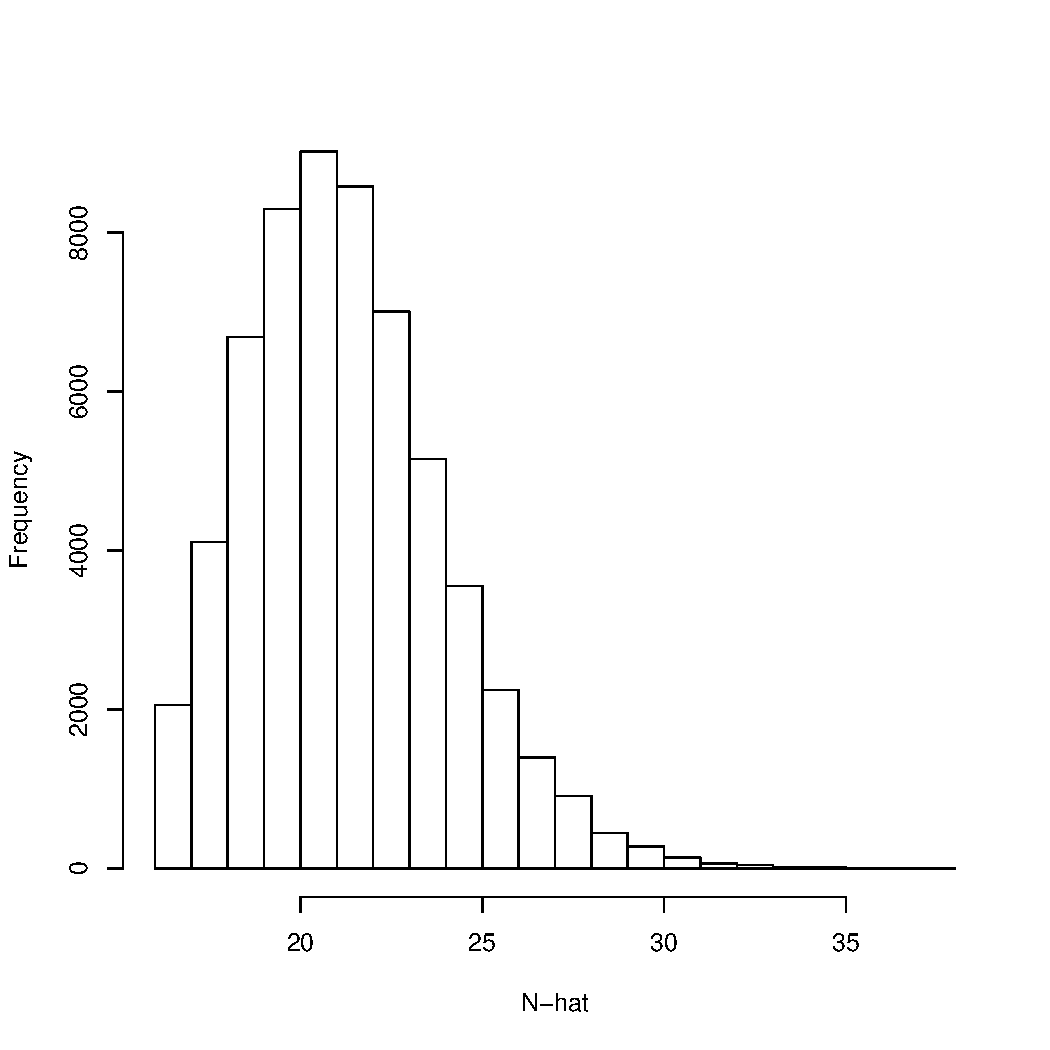
\includegraphics[height=2in,width=2.5in]{Ch12/figs/Nhat5ovenbird.pdf}
\caption{Histogram of $N_5$ from the spatial JS model for the ovenbird dataset.  This graph suggests that there is no truncation of the posterior of $N_5$. }
\label{open.figs.ovenbirdN5hist}
\end{figure}

In the JS formulation of the model, we also estimate the recruitment for each year,
and we can look at our derived values for recruitment (R2, R3, R4, and R5).
R2 is the number of new
recruits from primary period 1 to 2; R3 is the number of new recruits from primary period 2 to 3; and so forth.
R2 and R3 are almost
double that of R4 and R5, suggesting that less animals were recruited into the population in the latter years
of the study.  The density in
the last year of the study was lower than previous years.
It is good to check your results when you see a pattern like this -- the number
of recruits declining each year -- because this could be an indication that the data augmentation was not large enough.
In this example,
we checked to make sure that M=200 was sufficiently large by examining the recruitment parameter,
$\gamma$.  If $\gamma$ is close to 1 during any of the time periods, then there are not enough
augmented individuals in the overall dataset.  In this case, the 97.5\% quantile of $\gamma_5$, 
the recruitment probability in the final year of the study, was 0.14 and none of the other $\gamma$s
 were close to 1 either.  You can also look at the posterior distributions of $N$ to make sure 
they are not truncated, Fig. \ref{open.figs.ovenbirdN5hist} shows that the posterior distribution of $N_5$ is not 
truncated. The posterior mean for survival, $\phi$, was 0.53.  Although we did not do it here,
it should be easy to see that we could allow survival to vary by time, as we did with recruitment.
Our estimates of survival seem
reasonable when compared with the literature.  Some studies have found annual male ovenbird
survival to be around 0.62 \citep{porneluzi_faaborg:1999, bayne_hobson:2002}; however, 
female ovenbird
survival was much lower (0.21,
\cite{bayne_hobson:2002}). With more individuals, we could run this model with survival 
estimated for each sex separately.
However, we should be careful not to over-parameterize our model based on the amount of 
data available.

\section{Traditional CJS models}

The Cormack-Jolly-Seber models are used extensively in the literature to
determine detection and survival probabilities.  There are essentially two ways to
fit these models, using either a
multinomial approach \citep{lebreton_etal:1992} or a state-space
likelihood approach \citep{gimenez:2007, royle:2008}.

We can adopt a simple hierarchical parameterization of the
basic single state, non-spatial CJS model in which the observation model is
described conditional on the latent state variables $z(i,t)$ -- the
�alive state� � which describe whether individual $i$ is
alive ($z(i,t)=1$) or not ($z(i,t)=0$) during each of $t=1,2,\ldots,T$
{\it primary} periods.  Let $y_{it}$ indicate the observed
encounter data of individual $i$ in primary period $t$. The
model, specified conditional on $z(i,t)$, is:
 \[
  y_{it}|z_{it} \sim
\mbox{Bernoulli}(p_{t}z_{it}).
\]
Analogous to the JS model, if individual $i$ is alive at time $t$ ($z_{it}=1$),
then the observations are Bernoulli with probability of detection $p_t$.
If the
individual is not alive ($z_{it}=0$), then the observations must be
fixed zeros with probability 1.
In the CJS formulation, as opposed to the JS, we condition on first capture which means that $z_{it}$ will
be 1 when $t$ is the first primary period of capture.   We can denote this $z_{i f_i}$
where $f_i$ indicates the primary occasion in which individual $i$ is first captured, which 
can vary from $1 \dots T$.
This ensures that each individual is alive upon entering the model.

We can
describe the ''alive state" at time $t$ for each individual as a
function of the state at the previous time step $t-1$.   Because
we condition on the first capture, the initial
state is set to one:
\[
 z_{i f_i} = 1
\]
and to model the transition of individual states from $t$ to $t+1$ for
all $t > f_i$ we have
\[
 z_{i t} \sim \mbox{Bernoulli}( \phi z_{i,t-1}).
\]
Because we start with $z_{i f_i} = 1$, the individual survives with probability
$\phi$ to time $f_i + 1$ and so forth.  Once an individual leaves the
population (i.e., $z_{it} = 0$), there is no mechanism for the
individual to return.  This means that under this specification individuals cannot
temporarily emigrate.  In the CJS model we are not estimating $N$, so we do not incorporate
any data augmentation here.  This version of the model is easy to construct in the \bugs~ (or \jags~)
language which is shown in Panel \ref{open.panel.nsCJS}.  Variations on this basic model and associated code for
fitting the model in \bugs~ are described in detail in \citet[][Chapts. 7-9]{kery_schaub:2011}.

\begin{panel}[htp]
\centering
\rule[0.1in]{\textwidth}{.03in}
%\begin{minipage}{2.5in}
{\small
\begin{Verbatim}[commandchars=\\\{\}]
model \{
phi \mytilde dunif(0,1)   #Survival (constant over time)

for(t in 1:T)\{
p[t] \mytilde dunif(0, 1)    #detection (varies with time)
\}

for (i in 1:M)\{
   z[i,first[i]] ~ dbern(1)
  for (t in (first[i]+1):T) \{
         tmp[i,t] <- z[i,t]*p[t]
           y[i,t] \mytilde dbern(tmp[i,t])
       phiUP[i,t] <- z[i,t-1]*phi
           z[i,t] \mytilde dbern(phiUP[i,t])
   \}
  \}
\}
\end{Verbatim}
}

\rule[-0.1in]{\textwidth}{.03in}
\caption{
\jags~ model specification for the non-spatial basic CJS model.}
\label{open.panel.nsCJS}
\end{panel}


\begin{figure}
\centering
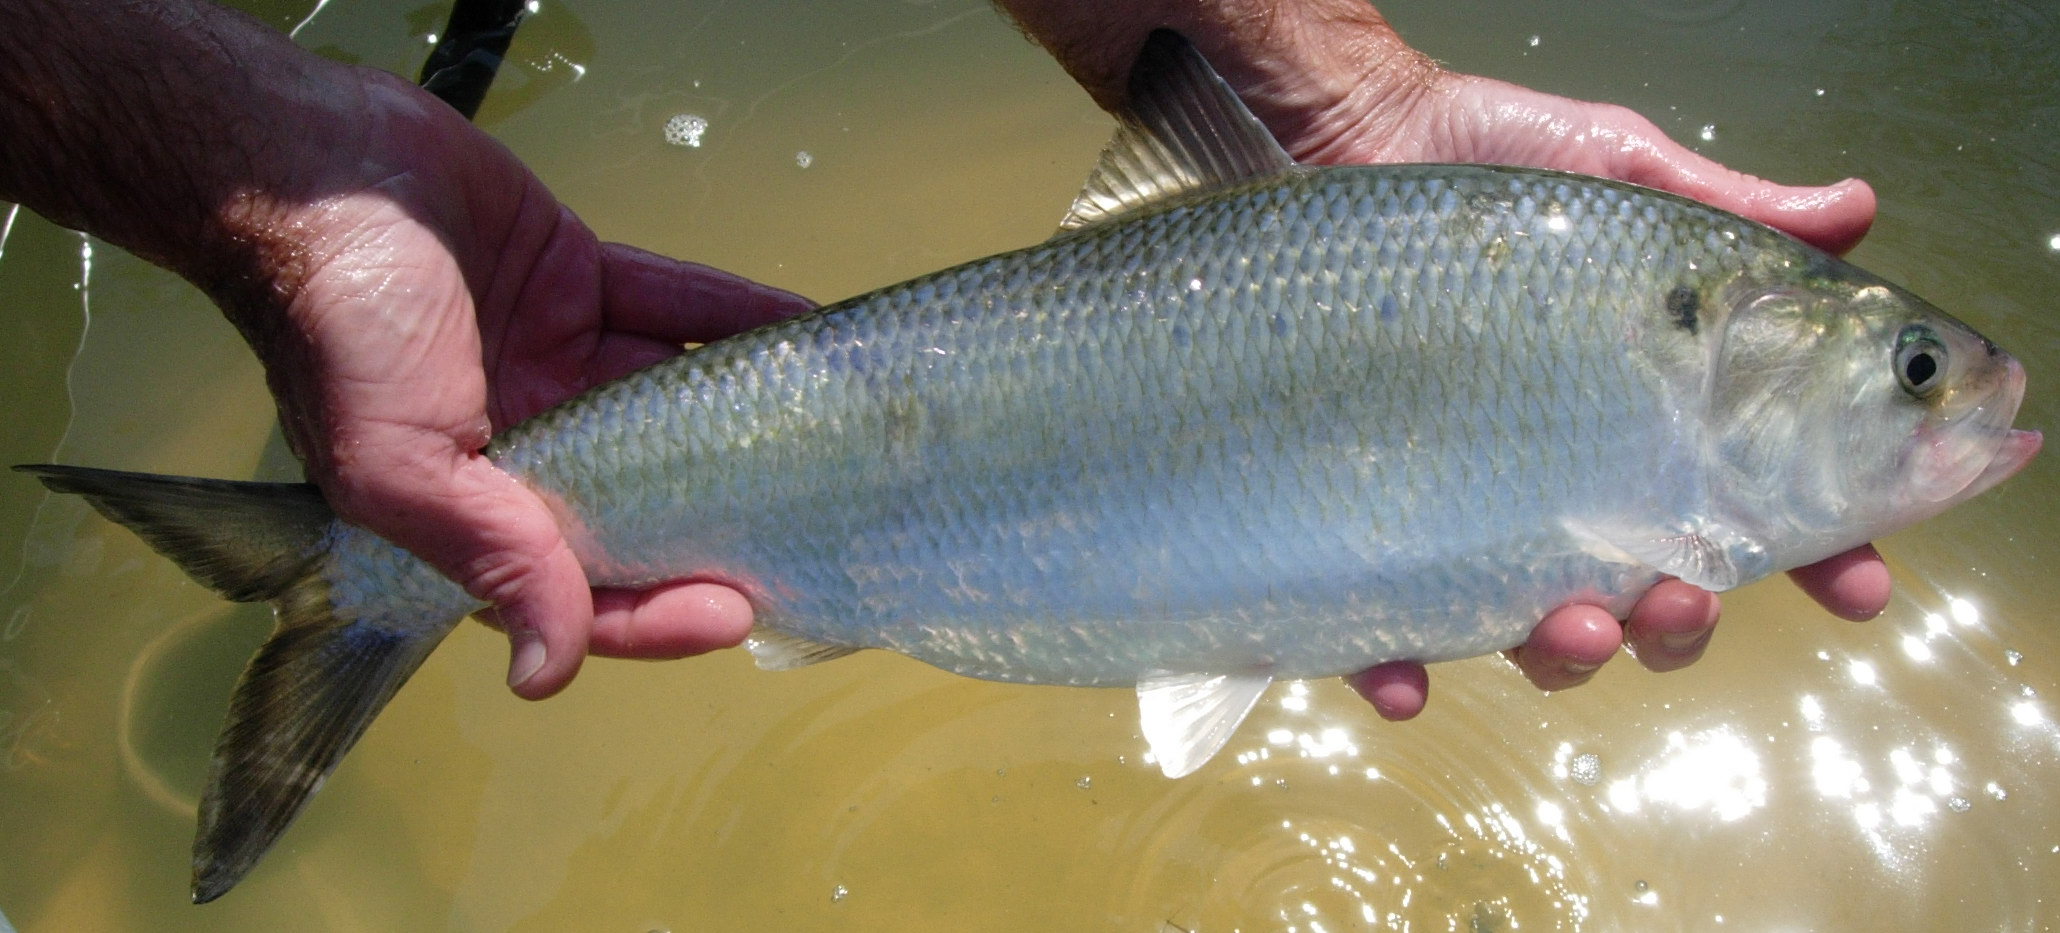
\includegraphics[height=2in,width=4.43in]{Ch12/figs/American_Shad_Raabe.jpg}
\caption{American shad caught in North Carolina, U.S.A.  Credit: Joshua Raabe, North Carolina State University}
\label{open.figs.shadpic}
\end{figure}

\subsection{Migratory fish example}
The motivation for this example stems from an interest in better
understanding survival and movement of migratory fishes.  For this
example, we will use data collected on American shad \textit{Alosa sapidissima}
in the New River in North Carolina, U.S.A. (see photo in Fig. \ref{open.figs.shadpic}).
The data were collected and analyzed in \cite{raabeDissertation:2012}. 
Using a resistance board weir near the
river mouth, 315 fish
were tagged with passive integrated transponders (PIT) in the spring
of 2010 . An array of 7 upstream PIT antennas passively recaptured
individuals during upstream and downstream migrations.  Each time a fish passed
over the antenna, it was recorded and summarized weekly for 12 weeks.  
To apply the basic CJS model, we create the
encounter history for each individual for the 12 weeks and we also create
a vector to indicate the period of first capture.

\begin{table}
\centering
\caption{Results of the basic non-spatial CJS model for the American shad dataset.
}
\begin{tabular}{crrrrr}
\hline \hline
&    Mean   &  SD  &  2.5 \%   &   50 \%    &  97.5 \% \\
p[1] & 0.499 & 0.289 & 0.026 & 0.499 & 0.975 \\
p[2] & 0.627 & 0.058 & 0.511 & 0.628 & 0.738 \\
p[3] & 0.762 & 0.036 & 0.689 & 0.763 & 0.829 \\
p[4] & 0.880 & 0.025 & 0.828 & 0.882 & 0.925 \\
p[5] & 0.548 & 0.043 & 0.465 & 0.548 & 0.633 \\
p[6] & 0.259 & 0.038 & 0.190 & 0.258 & 0.337 \\
p[7] & 0.126 & 0.031 & 0.072 & 0.124 & 0.194 \\
p[8] & 0.236 & 0.045 & 0.155 & 0.234 & 0.332 \\
p[9] & 0.237 & 0.049 & 0.148 & 0.234 & 0.341 \\ 
p[10]& 0.589 & 0.072 & 0.447 & 0.590 & 0.728  \\
p[11]& 0.834 & 0.063 & 0.700 & 0.839 & 0.942 \\
p[12]& 0.468 & 0.072 & 0.330 & 0.466 & 0.614 \\
$\phi$  & 0.824 & 0.011 & 0.802 & 0.825 & 0.846 \\
\hline
\end{tabular}
\label{open.tab.simple-shad}
\end{table}

Table \ref{open.tab.simple-shad} shows the estimated detection probability for each of the 12 primary periods
in the study.  The posterior mean for detection probability ranges from 0.126 to 0.880, which could potentially 
be due to variation in water flow, stream depth, storms, etc.  The weekly survival probability, $\phi$ had a
posterior mean estimate of 0.824.  This estimate could be considered low for a weekly probability, but 
is likely due to the fact
that the migration upstream can be quite energetically taxing.
Additionally, the CJS model is only estimating the 'apparent' survival
and some fish may have left the stream temporally or permanently. We demonstrate in panel \ref{open.panel.nsCJS} 
how to allow $p$ to vary by time, but we could also allow survival, $\phi$ to vary by time by 
implementing it exactly as 
we do $p$.
As we move into the multi-state model, 
we can test for movement and survival by state, allow us to address more specific biological questions.



\section{Multi-state CJS models}

The basic version of the CJS model only allows for estimation of survival and detection.  However,
researchers are often interested in addressing other ecological questions such as age-dependent
survival rates, habitat based movements, etc.  Multi-state models allow researchers to directly
address such questions by incorporating more than one state that an individual may potentially
be in \cite{arnason:1972,arnason:1973, brownie_etal:1993}.  These possible states can be geographic
location, age class, or reproductive status among many
others.  Instead of just having an encounter history for an individual, we will also have auxiliary
information on the state of that individual at capture (e.g., breeder or non-breeder).
Since our interest in movement of individuals, here we will consider states that represent spatial units or
geographic locations.  Generally speaking, we might think that the transition rates between locations could be due to
habitat features (or quality) and we can use multi-state models to help us address such a question.
In addressing movement through a multi-state modeling approach, the movement is often parameterized
as random or Markovian between patches (\cite{arnason:1972,arnason:1973, schwarz_etal:1993}).

In the simplest version of the multi-state model we have just two states.  Thus, individuals
can be marked and recaptured in one of two states (we'll call them A and B here).  
We will assume that the two ``states'' are different
geographic sites.  
In our single-state model above, an individual $i$ was either alive ($z_{it}=1$) at time $t$
or dead ($z_{it}=1$).  Now, we must consider that the individual could be alive in a given state or
dead and that individuals can transition between states.  An easy way to think about this is to look at
the state transition matrix in Table \ref{open.tab.CJSmulti-matrix}.  Here, $\phi_A$ is the probability of surviving
in State A from time $t$ to $t+1$ and $\phi_B$ is analogous for State B.  The 
movement parameters are $\psi_AB$ and $\psi_BA$,
where $\psi_AB$ is the probability that an individual, which survived 
from $t$ to $t+1$ in Site A, moves to State B just
before $t+1$ and vice versa for $\psi_BA$


\begin{table}[htb!]
\centering
\caption{
Transition matrix for a multi-state model with just two states.
}
\begin{tabular}{crrr}
\hline \hline
    &   State A &   State B   &   Dead \\  \hline
State A & $\phi_A(1-\psi_{AB})$ & $\phi_A \psi_{AB}$ & 1 - $\phi_A$ \\
State B & $\phi_B \psi_{BA}$ & $\phi_B(1-\psi_{BA})$ & 1 - $\phi_B$ \\
Dead & 0 & 0 & 1\\ \hline
\end{tabular}
\label{open.tab.CJSmulti-matrix}
\end{table}

We do not necessarily observe individuals in their given state though, so we must estimate detection
separately for each of the states.  Hence we also have $p_A$ and $p_B$, the probability of detecting
an individual in state A and state B respectively.

To relate this back to the description of multi-state models in Chapt. \ref{chapt.poisson-mn}, we can define ${\bf s}$
as the index of which state an individual is in and $u_{it}$ as
the state in which individual $i$ was observed during sample $t$.  In this two state example,
$u_{it}$ can only take on values for being observed in A or B (i.e., 1 or 2).

We can define a simplistic model where the successive movement outcomes
are $iid$
\[
u_{it} \sim  dcat( {\psi}({\bf s}_{i}) )
\]

Conditional on the state in which individual $i$ is located, we
observe that individual with probability $p_{0}$. That is:
\[
 \Pr(y_{it} = 1| u_{it} )  = p_{0}
\]
The state-transition
probabilities are constant, conditional on ${\bf s}$.  Other models for these transition probabilities
are possible and we will discuss those later.

To program this model in \jags, we use a slightly different formulation which essentially combines
$u_{it}$ and $y_{it}$ as defined above into one observation matrix such that $y_{it} = 1, 2,$ or $3$ where
3 indicates ``not observed''.  Additionally, we use $z_{it}$ to indicate the true state of individual
$i$ such that $z_{it} = 1, 2,$ or $3$ where 1 indicates alive and in state 1, 2 indicates alive and in state 2,
and 3 indicates ``not alive''.  Using this delineation, we just need to set up the transition
matrix based on Table \ref{open.tab.CJSmulti-matrix}
and define each item within the model specification, shown in Panel \ref{open.panel.msCJS}.
Note that this can become quite cumbersome when dealing with models that
have many states.


\begin{panel}[htp]
\centering
\rule[0.1in]{\textwidth}{.03in}
%\begin{minipage}{2.5in}
{\small
\begin{Verbatim}[commandchars=\\\{\}]
model \{
for(r in 1:2)\{
phi[r] \mytilde dunif(0,1)
psi[r] \mytilde dunif(0,1)
p[r] \mytilde dunif(0,1)
\}

for (i in 1:M)\{
    z[i,first[i]] <- y[i, first[i]]
for (t in (first[i]+1):T)\{
    z[i,t] \mytilde dcat(ps[z[i,t-1], i, ])
    y[i,t] \mytilde dcat(po[z[i,t], i, ])
\}
	ps[1, i, 1] <- phi[1] * (1-psi[1])
	ps[1, i, 2] <- phi[1] * psi[1]
	ps[1, i, 3] <- 1-phi[1]
	ps[2, i, 1] <- phi[2] * (1-psi[2])
	ps[2, i, 2] <- phi[2] * psi[2]
	ps[2, i, 3] <- 1-phi[2]
	ps[3, i, 1] <- 0
	ps[3, i, 2] <- 0
	ps[3, i, 3] <- 1

	po[1, i, 1] <- p[1]
	po[1, i, 2] <- 0
	po[1, i, 3] <- 1-p[1]
	po[2, i, 1] <- 0
	po[2, i, 2] <- p[2]
	po[2, i, 3] <- 1-p[2]
	po[3, i, 1] <- 0
	po[3, i, 2] <- 0
	po[3, i, 3] <- 1
\}
\}
\end{Verbatim}
}

\rule[-0.1in]{\textwidth}{.03in}
\caption{
\jags~ model specification for a two state version of the multi-state CJS model. Code adjusted
from \cite[][Chapt. 9]{kery_schaub:2011}. }
\label{open.panel.msCJS}
\end{panel}


\subsection{Migratory fish example}

Previously, we considered the American shad example for the most basic CJS model.  However, in 
this case, the researchers were interested in movement of fish during migration and so we
classified the stream into 2 states - ``downstream" and ``upstream".  Each antenna was assigned
to a state based on the location, those below 20 river kilometers were considered in 
the downstream state.  Each fish has an encounter history including whether or not the fish was
detected during each week of the 12 week study, but also the ``state" of capture 
(``downstream" or ``upstream").  Again, a vector to indicate the period of first capture was also
created.  Fish captured in more than one state during the week were assigned the state in which they were captured most during that week.   


\begin{table}
\centering
\caption{
Results of the multi-state CJS model for the migratory fish example.  $p_A$ is the detection probability in the first state (A), which in this case is the down stream area.  $phi_A$ is the weekly survival probability in state A and $\psi_AB$ is the probability that an individual, which survived from $t$ to $t+1$ in Site A, moves to State B just
before $t+1$. 
}
\begin{tabular}{crrrrr}
\hline \hline
&       Mean   &  SD  &  2.5 \%   &   50 \%    &  97.5 \%  \\  \hline
$p_A$ & 0.777 & 0.045 & 0.689  & 0.777  & 0.866 \\
$p_B$  & 0.434  & 0.027 & 0.382 & 0.434  & 0.489 \\
$\phi_A$  & 0.850 & 0.022 & 0.807  & 0.851  & 0.893  \\
$\phi_B$  & 0.782  & 0.019 & 0.743  & 0.782& 0.820  \\
$\psi_AB$ & 0.421 & 0.034 & 0.356  & 0.421 &  0.489 \\
$\psi_BA$& 0.927 & 0.014 & 0.897  & 0.937 &  0.952  \\

\hline
\end{tabular}
\label{open.tab.multi-shad}
\end{table}

Survival between the two areas is quite different (see Table \ref{open.tab.multi-shad}).  This might suggest that 
fish moving further upstream are expanding more energy and are more likely to die.  
While survival in the two states was different, it is intuitive that the average of the survival 
probabilities for A and B is essentially the same as that from the basic non-spatial CJS ($\phi = 0.82$, see Table \ref{open.tab.simple-shad}).   Also, it should be noted 
that $\psi_BA$ is very high indicating that fish in this study are returning downstream after spawning in the upstream area.
 These results highlight the utility in using a multi-state model to understand movement between states; here, 
we used spatial states, but age, class, breeding status, etc. are all possibilities.  We did have to reduce the 
dataset however to fit this model and information on spatial location was lost in creating just two states, downstream and upstream.  

\section{Spatial CJS models}

In Chapt. \ref{chapt.poisson-mn}, we describe how SCR models are
a essentially a type of multi-state model with spatially structured transition probabilities.
As we noted, individuals can appear in $>1$ states, simultaneously,
which is not directly analogous to a standard multi-state model.  However, building on the state-space and
multi-state CJS models, we can
explicitly incorporate individual movement as an
individual covariate model \citep{royle_indcov:2007}.
To move from the basic and multi-state CJS models to the SCR version, we need only make a few
changes to the model.  Essentially, we will not have discrete states and thus the biggest
difference is that individuals do not ``transition'' between a finite set of states, but
instead are allowed to move in continuous space.


We may consider the same basic encounter
models as described previously (i.e., Poisson, Bernoulli, or
multinomial). In particular, let $y_{ijkt}$ indicate the observed
encounter data of individual $i$ in trap $j$, during interval
(secondary period or sub-sample) $k=1,2,\ldots,K$ and primary period $t$. We note that in
some cases we may have intervals ($K=1$) which correspond to the
design underlying a standard CJS or JS models whereas the case $K>1$
corresponds to the ``robust design'' (\citealt{pollock:1982}).  The
Poisson observation model, specified conditional on $z(i,t)$, is:
 \[
  y_{ijkt}|z(i,t) \sim
\mbox{Poisson}(\lambda_0 g_{ij} z(i,t)).
\]
If individual $i$ is alive at time $t$ ($z(i,t)=1$), then the observations are Poisson as before.
Conversely, if the
individual is not alive ($z(i,t)=0$), then the observations must be
fixed zeros with probability 1.   In the CJS formulation, we will condition on first capture
which means that $z(i,t)$ will
be 1 when $t$ is the first primary period of capture.  We can denote this $z(i, f_i)$
where $f_i$ indicates the primary occasion in which individual $i$ is first captured.
This ensures that each individual is alive upon entering the model.   Modeling time-effects either
within or across primary periods
is straightforward. For that, we define $\lambda_{0} \equiv
\lambda_{0}(k,t)$ and then develop models for
$\lambda_{0}(k,t)$ as in our closed SCR models (we note that
trap-specific effects could be modeled analogously).

We follow the same model for survival as described in the non-spatial version of the
CJS.  The model is initialized by setting the alive
state at first capture to one:
\[
 z(i,f_i) = 1
\]
and for the transition of an individual's alive state from $t$ to $t+1$, for
all $t > f_i$, we have
\[
z_{it} \sim \mbox{Bernoulli}( \phi z_{i,t-1}).
\]
An individual survives with probability
$\phi$ from one time step to the next.  It is easy to see that we can let
survival be time specific by allowing $\phi$ to vary with each time step:
\[
 z_{it} \sim \mbox{Bernoulli}( \phi_t z_{i,t-1}).
\]

In either case, once an individual leaves the
population (i.e., $z_{it} = 0$), there is no recruitment so individuals cannot
return.  Again, we are not estimating $N$ in this model, hence we do not need
any data augmentation.  This conveniently makes the model run
faster too!


\subsection{Migratory fish example}

Going back to our American shad example, we can consider that this is
exactly a spatial capture recapture problem. 
In stream networks, the placement of PIT antennas along the stream mimics the
type of spatial data collected in terrestrial passive detector arrays such as
camera traps, hair snares, acoustic recording devices, etc.  The
difference is that for fish and aquatic species, the stream constrains
the movement of individuals to a linear network.  Using the data from the
array of 7 PIT antennas and the number of
times each fish passed over the antenna, we can apply the SCR CJS model to
evaluate movement up and downstream of these fishes.
When we look at the individuals encountered at each antenna for each of the primary periods,
the dimensions of the data are 315
individuals by 7 antennas by 12 sample occasions. Individuals can
encounter any antenna any number of times during the week, which means
we just sum the encounters over the week and eliminate any need for
explicit secondary occasions in the model. The result is a 3-D array
instead of a 4-D array.  Given the structure of the encounters, we use
a Poisson encounter model in this example.


{\small
\begin{verbatim}
library(reshape)

# Constants:
M <- 315       # Number of individuals
T <- 12     # Number of periods (weeks)
nantenna <- 7  # weir, 6 antennas
antenna.loc <- c(3,7,12,44,56,72,77)  # antenna locations

# Input and format data matrix:
AS10 <- read.table("AS10.txt" ,header=T)
melted.rkm <- melt(AS10, id=c("TagID","RKM"))
y <- cast(melted.rkm, TagID ~ RKM ~ value, fill=0, length)
first=read.csv("firstcap.csv")

sink("ModelCJS.txt")
cat("

model {
# Priors
sigma ~ dunif(0,80)
sigma2 <- sigma*sigma
lam0 ~ dgamma(0.1, 0.1)
phi ~ dunif(0, 1)   # Survival (constant across time)
tauv~dunif(0, 30)
tau<-1/(tauv*tauv)

for (i in 1:M){
  z[i,first[i]] <- 1
  S[i,first[i]] ~ dunif(0,50)

for(j in 1:nantenna) {
	  D2[i,j,first[i]] <- pow(S[i,first[i]]-antenna.loc[j], 2)
       lam[i,j,first[i]]<-  lam0*exp(- D2[i,j,first[i]]/(2*sigma2))
       tmp[i,j,first[i]] <- lam[i,j,first[i]]
         y[i,j,first[i]] ~ dpois(tmp[i,j,first[i]])
      }

   for (t in first[i]+1:T) {
	          S[i,t] ~ dunif(xl, xu)
         for(j in 1:nantenna) {
		        D2[i,j,t] <- pow(S[i,t]-antenna.loc[j], 2)
               lam[i,j,t] <- lam0 * exp(-D2[i,j,t]/(2*sigma2))
	           tmp[i,j,t] <- z[i,t]*lam[i,j,t]
		         y[i,j,t] ~ dpois(tmp[i,j,t])
		 }
 	   phiUP[i,t] <-  z[i,t-1]*phi
	       z[i,t] ~ dbern(phiUP[i,t])
	}
	}
}

",fill = TRUE)
sink()

data1<-list(y=y, first=first, M=M, T=T, xl=0, xu=80, nantenna=nantenna, antenna.loc=antenna.loc)

z=matrix(NA, M, T)
for(i in 1:M){
for(t in first[i]:12){
z[i,t] <-1
}
}

inits =  function() {list(z=z,phi=runif(1,0,1), lam0=runif(1,0,2),
                     tauv=runif(1,10, 20), sigma=runif(1,0,10)) }

parameters <- c("sigma", "phi", "lam0")

library("rjags")
out1 <- jags.model("modelCJS.txt", data1, inits, n.chains=3, n.adapt=500)
out2CJS <- coda.samples(out1,parameters,n.iter=20000)
\end{verbatim}
}

\begin{table}
\centering
\caption{
Results of the spatial CJS model fitted to the
American shad data set.
}
\begin{tabular}{crrrrr}
\hline \hline
&       Mean   &  SD  &  2.5 \%   &   50 \%    &  97.5 \% \\
lam0[1] &  5.555& 0.224  & 5.125 & 5.553 	& 6.003 \\
lam0[2] &  4.442& 0.155  & 4.143 & 4.437  & 4.752 \\
lam0[3] &  1.892& 0.068  & 1.763 & 1.891  & 2.031 \\
lam0[4] &  1.126& 0.055  & 1.021 & 1.125  & 1.238 \\
lam0[5] &  0.949& 0.058  & 0.838 & 0.948 & 1.067 \\
lam0[6] &  0.359& 0.040  & 0.284 & 0.357 & 0.443 \\
lam0[7] &  0.188& 0.031  & 0.133 & 0.186 &  0.254 \\ 
lam0[8] &  0.309 &0.044  & 0.230  & 0.307  & 0.402 \\
lam0[9]  & 0.363 &0.052 &  0.269 &  0.361 & 0.471 \\
lam0[10] & 0.627 &0.072  & 0.493  & 0.625  & 0.777 \\
lam0[11] & 1.611 &0.109  & 1.408  & 1.607  & 1.835 \\
lam0[12] & 0.939 &0.139 & 0.697  & 0.929  & 1.241 \\
$\phi$  &  0.784 &0.012  & 0.760  & 0.785  & 0.807 \\
$\sigma$ & 13.954& 0.197  & 13.573 & 13.950  & 14.350\\

\hline
\end{tabular}
\label{open.tab.shad1}
\end{table}

The baseline encounter rate, $\lambda_0$, was allowed to vary by week and ranged from 0.188 to 5.555. 
We use the Poisson encounter model in this spatial CJS example rendering  $\lambda_0$ not directly
comparable to $p_0$ from the non-spatial and multi-state versions which arises as the detection probability
based under the Binomial encounter model. The
posterior mean estimate for $\phi$ was 0.784 (see Table \ref{open.tab.shad1}), again showing that the
survival probability is generally low, just as we saw in the two previous example analysis of these data.  
Here, we are modeling survival probability as constant, but there is reason to believe that it might vary by 
time (similar to detection) and we might consider this additional parameterization in a more 
complete analysis of the data set. The
other parameter of interest is $\sigma$, the movement parameter, which had a posterior mean of 13.954.  Our
system here is linear, so we do not think of fish as having a home
range radius in this system.  However, $\sigma$ can still inform us
about the linear distance fish are moving.


\section{Activity Centers}

We extend the model of individual encounter histories by specifying an
additional model component that describes the spatial distribution of
individual activity centers.  A plausible ``null model'' for the
distribution of individual activity centers is to assume they are
static over time and do not change across primary periods, 
i.e., ${\bf s}_{i} \sim \mbox{Unif}({\cal S})$.  It might seem more likely
that activity centers change over time but are independent from year to year for a 
giving individual such ${\bf s}_{i} \sim \mbox{Unif}({\cal S})$.  This is how 
the spatial version of the JS and CJS models were formulated above. 
Another option would be to assume that ${\bf s}(i,t) \sim \mbox{Normal}({\bf
  s}(i,t-1), \tau^{2} {\bf I})$ for $t > 1$ so that individual home range
centers are perturbed randomly from their previous value.

We could use this specification to model changes in habitat with regards to home range
centers.  If our primary period is season, we may expect that individuals move as
the available food sources change. Given that we have an indicator of habitat that varies by season,
we can model the location of activity centers as a function of the change in habitat.
For example, in our American shad example above, we have reason to believe
that individual movement is directly related to stream flow.  When the stream has
very low flow, we might expect that the fish move very little and when the stream
has a higher flow, the fish move upstream to spawn. In this case,
we could model the effect of stream flow in two ways.  First, we might allow $\sigma$
to be a function of flow and to vary for each primary ocassion.

\[
 \mbox{log}(\sigma_t) = \mu_S + \alpha_2 \mbox{Flow}_t
\]

But if we think that the change in activity centers might be related to the overall movement
of fish, then we could allow the variation in locations to be a function of flow.  Thus,
we might have
\[
{\bf s}(i,t) \sim \mbox{Normal}({\bf
  s}(i,t-1), \tau^{2} {\bf I})
\]
where
\[
\mbox{log}(\tau) = \mu_T + \alpha_2 \mbox{Flow}_t
\]

There are a number of options here for how we might allow activity centers to vary as a function
of covariates such as habitat, season, or behavior.  This is just the beginning of modeling how
the spatial arrangement of individuals within a study, we can also look at other point process models
such as the Strauss model, or we can use diffusion models to look at correlation between activity centers, etc..
XX this part should suggest that we are going to talk about the Otso papers. XXX



\subsection{Migratory Fish - Auto regressive model}




\section{Summary and Outlook}

Activity center dynamics..... A brief survey of the point process
literature to indicate what is out there......

There is a classical paper by Rathbun and Cressie









